\section{结构化输出的相关滤波跟踪}

\begin{frame}{工作点3}
    \tableofcontents[sections=\thesection]
\end{frame}

\subsection{算法简介}
\begin{frame}{算法简介}

\begin{block}{着眼问题}
相关滤波器利用傅里叶域特性能够高效地预测,但边界效应对跟踪性能有显著的影响。
\end{block}

\begin{block}{解决方案}
本章提出一种结构化输出的相关滤波跟踪方法,在利用相关滤波密集取样优势的同时,显著减少边界效应带来的性能损失。
\end{block}
\end{frame}


\subsection{有限边界的相关滤波器}

\begin{frame}{MOSSE相关滤波器}
MOSSE相关滤波器可以在空间域中表示为求解岭回归问题:
~\\
\begin{equation}
    E(h)= \frac{1}{2}\sum_{i=1}^N\sum_{j=1}^D\|y_i(j)-h^\top x_i[\Delta\tau_j]\|_2^2 + \frac{\lambda}{2}\|h\|_2^2
    \label{eq:CFwLB_MOSSEinSpatial}
\end{equation}
~\\
其中$y_i\in \mathbb{R}^D$是第$i$个观测$x_i\in \mathbb{R}^D$的期望响应,$\lambda$是正则项参数。$\mathbb{C} = [\Delta\tau_1,\dots,\Delta\tau_D]$表示长度为$D$的信号的所有循环移位集合。
\end{frame}

\begin{frame}{边界效应}

\begin{columns}
\centering
\column{0.7\linewidth}
\setlength{\parindent}{2\ccwd}

相关滤波器从由1个真实示例与其他合成示例组成的非平衡集合中估计出判别性模板。这些合成的样本是通过对真实样本应用循环移位来创建的。

~\\
如右图所示,循环移位的样本都受循环边界效应的影响,并不能代表真实的移动。边界效应可以显著影响所得到的估计模板,使得相关滤波器对平移中的偏差特别敏感。

\column{0.3\textwidth}
   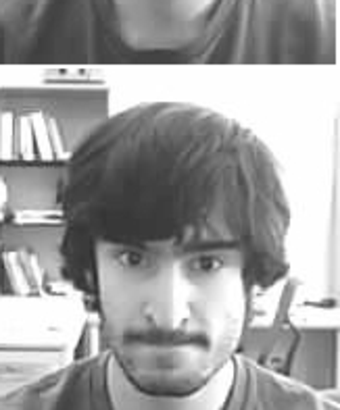
\includegraphics[width =\textwidth,height =1.3\textwidth]{CFwLB_a_3.pdf}
\end{columns} 
\end{frame}

\begin{frame}{引入掩蔽矩阵}
%%Boundary Effects

\begin{columns}
\centering
\column{0.65\textwidth}
\setlength{\parindent}{2\ccwd}

    有限边界滤波器能够在空间上避免边界效应。其训练信号$x\in \mathbb{R}^T$的大小比滤波器$h\in\mathbb{R}^D$大。通过使用掩蔽矩阵$P\in \mathbb{R}^{D\times T}$,可以将等式(\ref{eq:CFwLB_MOSSEinSpatial})表示为:
\column{0.3\linewidth}
   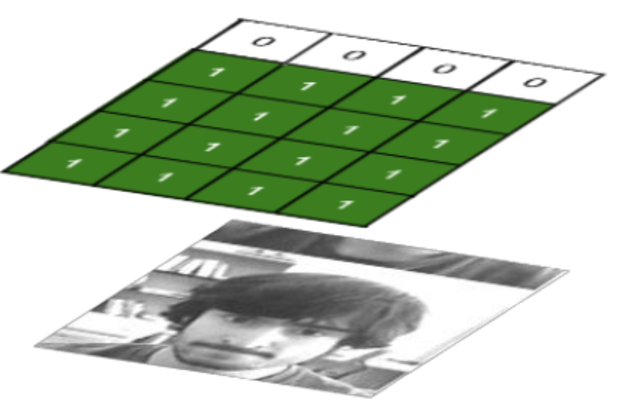
\includegraphics[width =\textwidth,height =0.7\textwidth]{MaskingMatrix.pdf}
\end{columns} 
~\\
\begin{equation}
    E(h)= \frac{1}{2}\sum_{i=1}^N\sum_{j=1}^T\|y_i(j)-h^\top Px_i[\Delta\tau_j]\|_2^2 + \frac{\lambda}{2}\|h\|_2^2
    \label{eq:CFwLB_MOSSEinSpatialwithMaskingMatix}
\end{equation}
~\\
掩蔽矩阵$P$封装了信号,其中的1和0决定哪一部分应该是有效的,哪一部分是无效的。

\end{frame}

\begin{frame}{样本对比}
\begin{figure}[htp]
\centering
\subfloat[传统滤波器样本]{
                          \begin{minipage}[b]{0.4\linewidth}
                          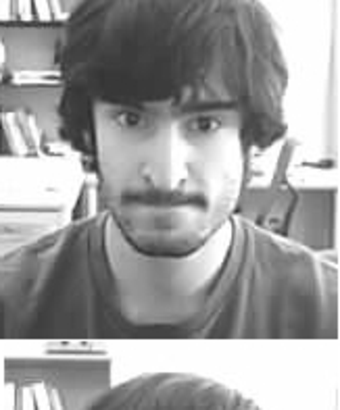
\includegraphics[width =0.3\linewidth,height =0.4\linewidth]{CFwLB_a_2.pdf}
                          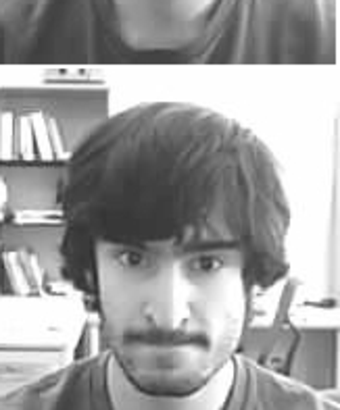
\includegraphics[width =0.3\linewidth,height =0.4\linewidth]{CFwLB_a_3.pdf}
                          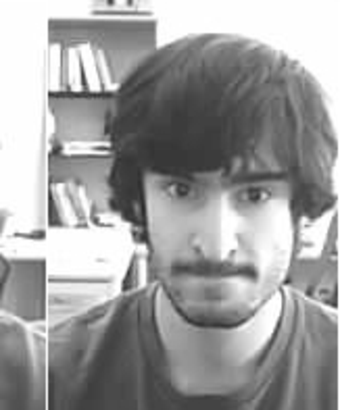
\includegraphics[width =0.3\linewidth,height =0.4\linewidth]{CFwLB_a_4.pdf}\\
                          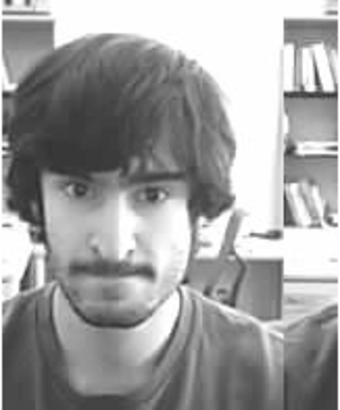
\includegraphics[width =0.3\linewidth,height =0.4\linewidth]{CFwLB_a_5.pdf}
                          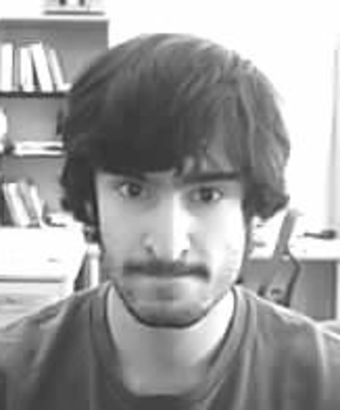
\includegraphics[width =0.3\linewidth,height =0.4\linewidth]{CFwLB_a_1.pdf}
                          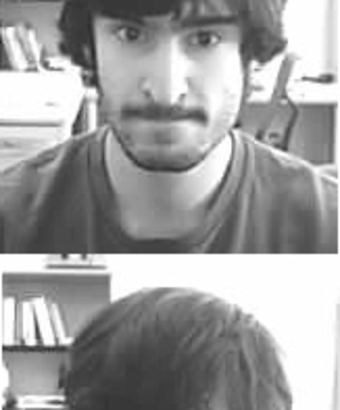
\includegraphics[width =0.3\linewidth,height =0.4\linewidth]{CFwLB_a_6.pdf}\\
                          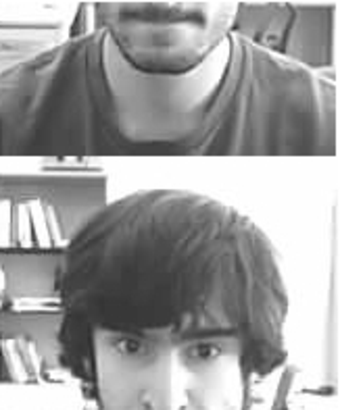
\includegraphics[width =0.3\linewidth,height =0.4\linewidth]{CFwLB_a_7.pdf}
                          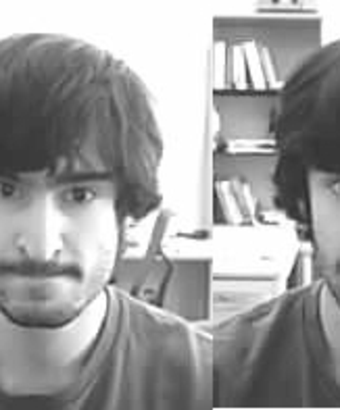
\includegraphics[width =0.3\linewidth,height =0.4\linewidth]{CFwLB_a_8.pdf}
                          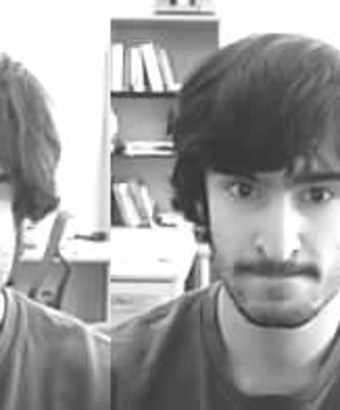
\includegraphics[width =0.3\linewidth,height =0.4\linewidth]{CFwLB_a_9.pdf}
                          \end{minipage}

\label{fig:CFwLB_CFSamples}}
\subfloat[有限边界滤波器样本]{
                              \begin{minipage}[b]{0.3\linewidth}
                              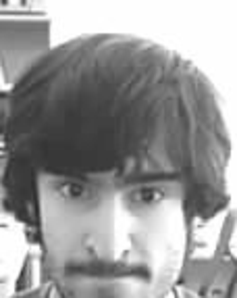
\includegraphics[width =0.3\linewidth,height =0.4\linewidth]{CFwLB_b_2.pdf}
                              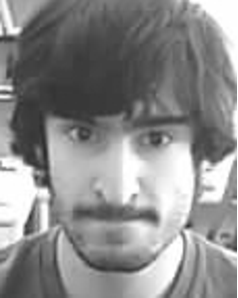
\includegraphics[width =0.3\linewidth,height =0.4\linewidth]{CFwLB_b_3.pdf}
                              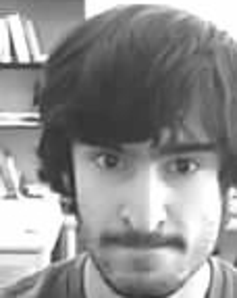
\includegraphics[width =0.3\linewidth,height =0.4\linewidth]{CFwLB_b_4.pdf}\\
                              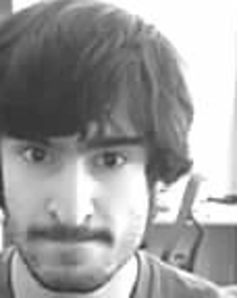
\includegraphics[width =0.3\linewidth,height =0.4\linewidth]{CFwLB_b_5.pdf}
                              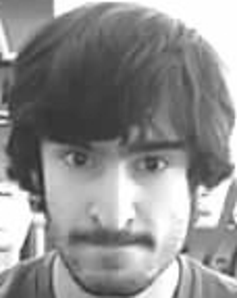
\includegraphics[width =0.3\linewidth,height =0.4\linewidth]{CFwLB_b_1.pdf}
                              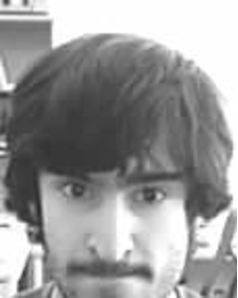
\includegraphics[width =0.3\linewidth,height =0.4\linewidth]{CFwLB_b_6.pdf}\\
                              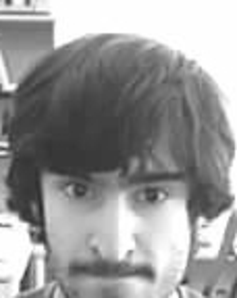
\includegraphics[width =0.3\linewidth,height =0.4\linewidth]{CFwLB_b_7.pdf}
                              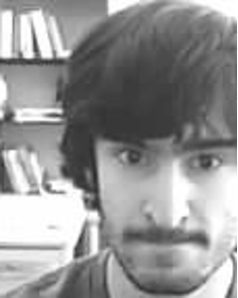
\includegraphics[width =0.3\linewidth,height =0.4\linewidth]{CFwLB_b_8.pdf}
                              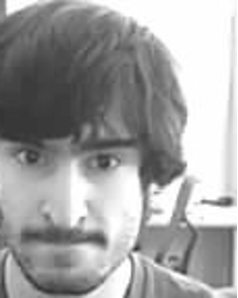
\includegraphics[width =0.3\linewidth,height =0.4\linewidth]{CFwLB_b_9.pdf}\\
                              \end{minipage}

\label{fig:CFwLB_Samples}}
\caption{有限边界滤波器}
\label{fig:CFwLB_Intro}
\end{figure}
\end{frame}

%\begin{frame}{滤波器的傅里叶域表示}
%等式(\ref{eq:CFwLB_MOSSEinSpatialwithMaskingMatix})可以在傅立叶域中表示为:
%~\\
%\begin{equation}
%E(h)= \frac{1}{2}\sum_{i=1}^N\sum_{j=1}^T\|\hat{y}_i(j)-\mathrm{diag}(\hat{x}_i)^\top\sqrt{D}FP^\top h]\|_2^2 + \frac{\lambda}{2}\|h\|_2^2
    %\label{eq:CFwLB_MOSSEwithMaskingMatixInFourier}
%\end{equation}
%~\\
%\end{frame}

%\begin{frame}{增强拉格朗日方法(ALM)}
%引入辅助变量$g$,等式(\ref{eq:CFwLB_MOSSEwithMaskingMatixInFourier})可以相同地表示为:
%~\\
%\begin{equation}
%\begin{aligned}
%E(h,\hat{g})& = \frac{1}{2}\sum_{i=1}^N\sum_{j=1}^T\|\hat{y}_i(j)-\mathrm{diag}(\hat{x}_i)^\top \hat{g}]\|_2^2 + \frac{\lambda}{2}\|h\|_2^2 \\
    %\mathrm{s.t.}\quad &\hat{g}= \sqrt{D}FP^\top h
    %\end{aligned}
    %\label{eq:CFwLB_objectiveFunction}
%\end{equation}
%~\\
%可以通过增强拉格朗日方法(Augmented Lagrange Method, ALM)来处理引入的等式约束。
%\end{frame}

%\begin{frame}{目标函数的ALM的表示}
%~\\
%\begin{equation}
%\begin{aligned}
%\mathcal{L}(\hat{g},h,\hat{\zeta})= &\frac{1}{2}\sum_{i=1}^N\|\hat{y}_i(j)-\mathrm{diag}(\hat{x}_i)^\top \hat{g}]\|_2^2 + \frac{\lambda}{2}\|h\|_2^2\\
                                    %&+ \hat{\zeta}^\top(\hat{g}-\sqrt{D}FP^\top h)\\
                                    %&+ \frac{\mu}{2}\|\hat{g}-\sqrt{D}FP^\top h\|_2^2
%\end{aligned}
    %\label{eq:CFwLB_augmented LagrangianObjectiveFunction}
%\end{equation}
%~\\
%其中$\mu$是控制ALM收敛速率的惩罚因子,$\hat{\zeta}$是在等式(\ref{eq:CFwLB_objectiveFunction})中强制引入的等式约束所需拉格朗日矢量的傅里叶变换。
%\end{frame}

\subsection{对于有限边界滤波器的改进}

\begin{frame}{标签图}
\begin{columns}
\centering
\column{0.4\textwidth}
\begin{figure}[htp]
  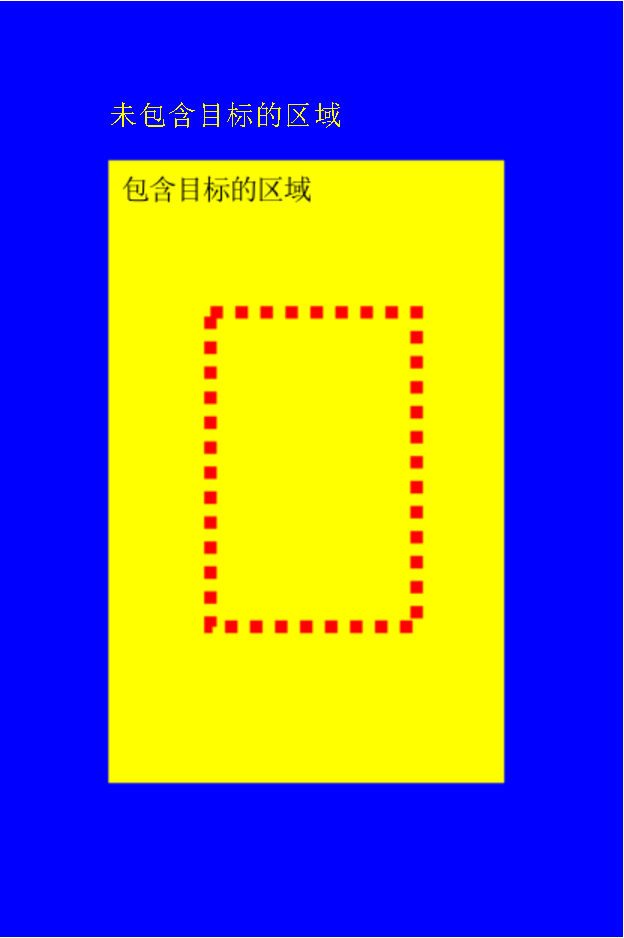
\includegraphics[height=.7\textheight]{figures/CFwLBlabels.pdf}
\caption{有限边界滤波器标签图}
\label{fig:CFwLB_labels}
\end{figure}

\column{0.6\textwidth}
\setlength{\parindent}{2\ccwd}

有限边界相关滤波器只对样本进行了加工,而未注意到样本与标签的匹配问题。由于扩大滤波器尺寸的同时仍采用了传统相关滤波器的平滑高斯函数生成标签,未包含目标的样本块同样被赋予了正标签。因而,滤波器无法学习到区分度高的特征。
\end{columns}
\end{frame}

\begin{frame}{以结构化方式定义样本}

借鉴图像检测中的结构化输出方法,以样本框的坐标作为样本标签,这使得样本描述与实际问题相一致。
~\\
\begin{equation}
E(h)= \frac{1}{2}\sum_{i=1}^N\sum_{j=1}^T\|\widehat{l(y_i(j))}-\mathrm{diag}(\hat{x}_i)^\top\sqrt{D}FP^\top h]\|_2^2 + \frac{\lambda}{2}\|h\|_2^2
    \label{eq:CFwLB_MOSSEwithMaskingMatixInFourierStructuredOutput}
\end{equation}
~\\
其中,评价函数$l(y)=\frac{\mathrm{Area}(y_i\cap y^\ast)}{\mathrm{Area}(y_i\cup y^\ast)}$表示样本框与目标框的重叠率,$y^\ast$为目标框的坐标表示,$\mathrm{Area}$表示求两个矩形框的面积。
\end{frame}

\subsection{实验结果}



%%%单元格中显示多行
\begin{frame}{距离精度(DP)}
\begin{table}[!t]
\centering
%%%增大行距
\renewcommand{\arraystretch}{1.3}
%\setlength{\abovecaptionskip}{15pt plus 3pt minus 2pt}
\captionsetup{belowskip=2pt,aboveskip=4pt}

\caption{20个像素偏差内的距离精度}
\begin{adjustbox}{max width=\textwidth}
    \begin{tabular}{|c|c|c|c|c|c|c|c|c|}
        \hline
        Sequance  & Frag  &  OAB  &  SBT  &  MIL  & Struck & CSK   & CFwLB   &  Ours \\ \hline
        
        Coke      & 0.034 & 0.168 & 0.048  & 0.117 & \textcolor{blue}{0.942} & 0.739 & 0.918   & \textcolor{red}{0.959}  \\ \hline
        David     & 0.121 & 0.151 & 0.204  & 0.229 & \textcolor{blue}{0.236} & \textcolor{blue}{0.236} & 0.144   & \textcolor{red}{0.396} \\ \hline
        Dog       & 0.173 & 0.157 & 0.079  & 0.197 & 0.157 & 0.144 & \textcolor{blue}{0.858}   & \textcolor{red}{0.992}  \\ \hline
        Doll      & 0.663 & 0.663 & 0.149  & 0.433 & 0.688 & 0.218 & \textcolor{blue}{0.947}& \textcolor{red}{ 0.986} \\ \hline
        Gym       & \textcolor{blue}{0.369} & 0.016 & 0.046  & 0.329 & 0.219 & 0.091 & 0.113   & \textcolor{red}{0.801}  \\ \hline
        KiteSurf  & 0.143 & 0.381 & 0.369  & 0.381 & \textcolor{blue}{0.905} & 0.321 & 0.274   & \textcolor{red}{0.964}  \\ \hline
        Surfer    & 0.176 & 0.045 & 0.133  & 0.088 & 0.157 & 0.005  & \textcolor{blue}{0.468}   & \textcolor{red}{0.997}  \\ \hline
    Sylvester     & 0.685 & 0.680 & 0.430  & 0.546 & \textcolor{blue}{0.929} & 0.717 & 0.921 & \textcolor{red}{0.947}\\ \hline
        Vase      & 0.166 & 0.155 & 0.129  & 0.166 & 0.140 & 0.166  & \textcolor{blue}{0.181}   & \textcolor{red}{0.657}  \\ \hline \hline

        mean      &0.281  & 0.268 & 0.176  & 0.276 & 0.486 & 0.293  & \textcolor{blue}{0.536}& \textcolor{red}{0.855} \\ \hline
\end{tabular}
\end{adjustbox}
\label{tab:CFwLB_precision}
\end{table}
\end{frame}

\begin{frame}{中心位置误差(CLE)}
\begin{table}[htbp]
\centering
\renewcommand{\arraystretch}{1.3}
\captionsetup{belowskip=2pt,aboveskip=4pt}

\caption{平均中心位置误差}
\begin{adjustbox}{max width=\textwidth}
    \begin{tabular}{|c|c|c|c|c|c|c|c|c|}
        \hline
        Sequance  & Frag  &  OAB  &  SBT  &  MIL  & Struck & CSK   & CFwLB   &  Ours \\ \hline
        
        Coke      & 124.8 & 35.9  & 365.3 & 46.7  &  \textcolor{red}{12.1}  & 13.6  & 13.2   &   \textcolor{blue}{12.9}  \\ \hline
        David     & 82.1  & 21.7  & 47.1  & \textcolor{red}{16.9}  & 42.8   &  \textcolor{blue}{17.7} & 73.6   &   28.9  \\ \hline
        Dog       & 12.2  & 10.7  & 172.5 & 8.2   &  10.4  &  \textcolor{blue}{7.0}  & 11.8   & \textcolor{red}{6.8}  \\ \hline
        Doll      & 13.7  & 12.4  & 113.9 & 16.7  & \textcolor{blue}{8.9}&  44.7 & 9.5    & \textcolor{red}{ 4.6} \\ \hline
        Gym       & 10.0  & 111.0 & 230.4 & 11.8  & 18.5   &  27.1 & \textcolor{blue}{9.5}  & \textcolor{red}{ 4.6} \\ \hline
        KiteSurf  & 141.1 & 64.6  & 32.9  & 22.6  & \textcolor{red}{6.1}   &  36.5 & 85.7    & \textcolor{blue}{10.6} \\ \hline
        Surfer    & 51.6  & 72.1  & 218.5 & 17.0  &\textcolor{blue}{9.0}   & 161.7 & 25.3    & \textcolor{red}{6.5} \\ \hline
        Sylvester & 15.0  & 14.8  & 101.5 & 15.2  &\textcolor{red}{6.3}  &  9.9  & 8.8    & \textcolor{blue}{7.0} \\ \hline
        Vase      & 18.2  & 34.7  & 172.3 & 19.0  &  24.3   & \textcolor{red}{12.9} & 59.7    & \textcolor{red}{16.7} \\ \hline \hline

    mean      & 52.1  &  52.0 & 161.6 & 19.3  & \textcolor{blue}{15.4}  & 36.8 & 33.0 & \textcolor{red}{11.0} \\ \hline

\end{tabular}
\end{adjustbox}
\label{tab:CFwLB_CLE}
\end{table}
\end{frame}

\begin{frame}{中心位置误差对比}
\begin{figure}[htbp]
\centering
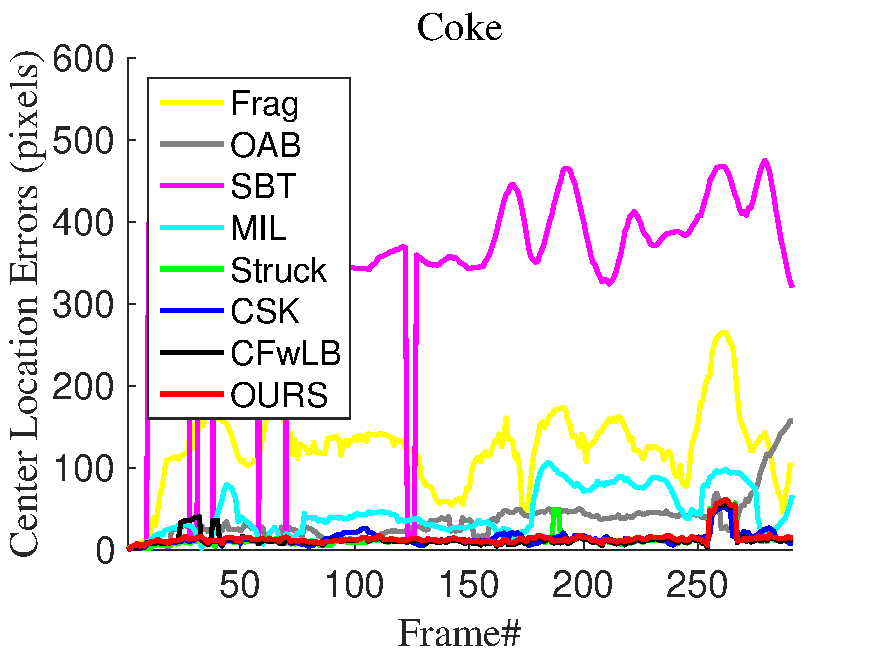
\includegraphics[width=0.3\linewidth]{CFwLB_Coke_prcision.pdf}
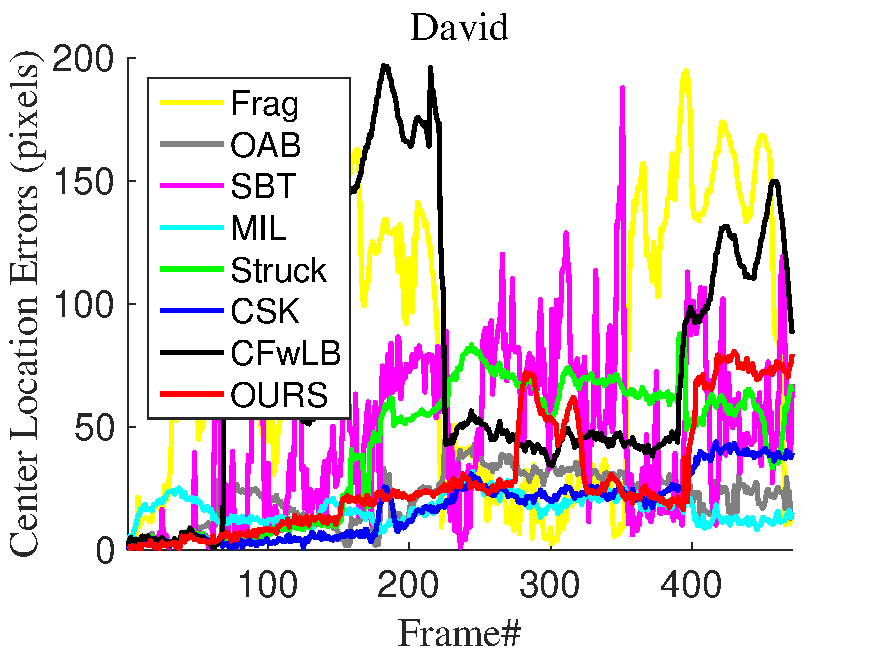
\includegraphics[width=0.3\linewidth]{CFwLB_David_prcision.pdf}
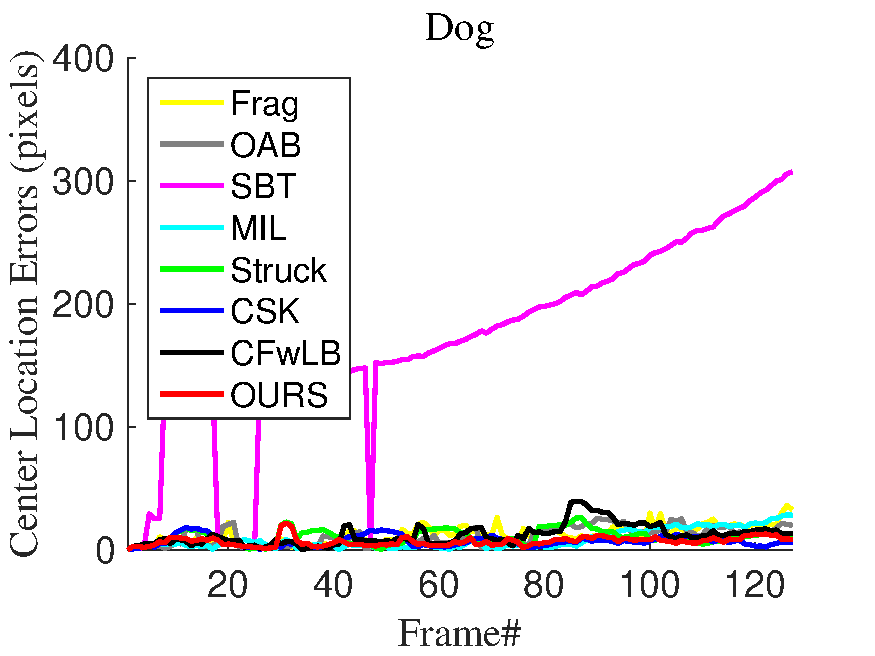
\includegraphics[width=0.3\linewidth]{CFwLB_Dog_prcision.pdf}\\
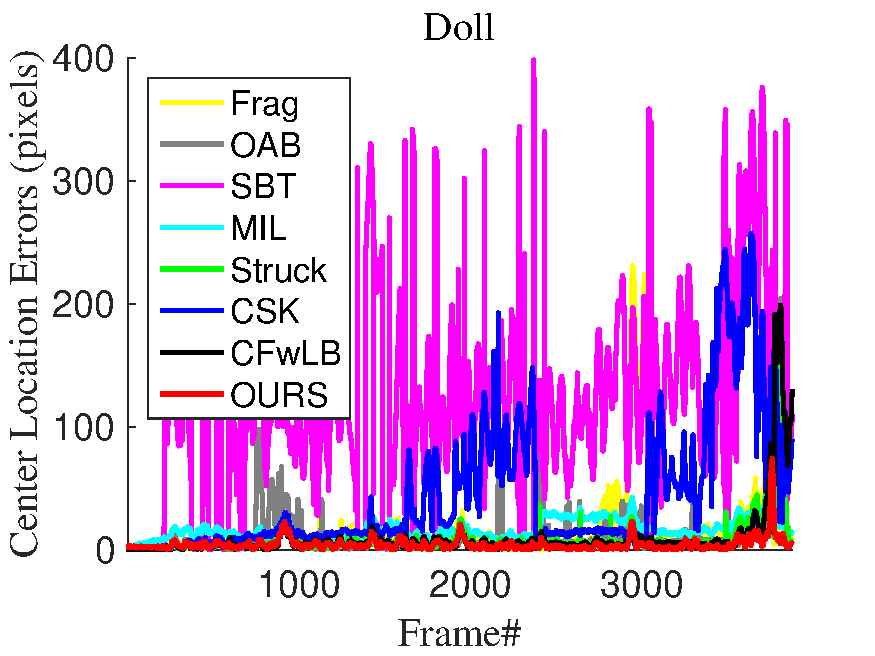
\includegraphics[width=0.3\linewidth]{CFwLB_Doll_prcision.pdf}
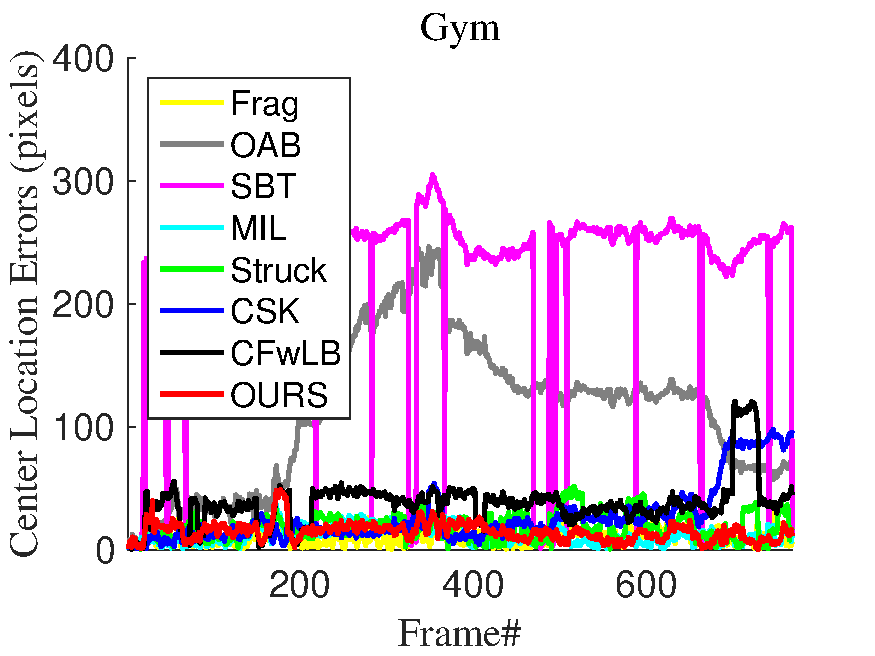
\includegraphics[width=0.3\linewidth]{CFwLB_Gym_prcision.pdf}
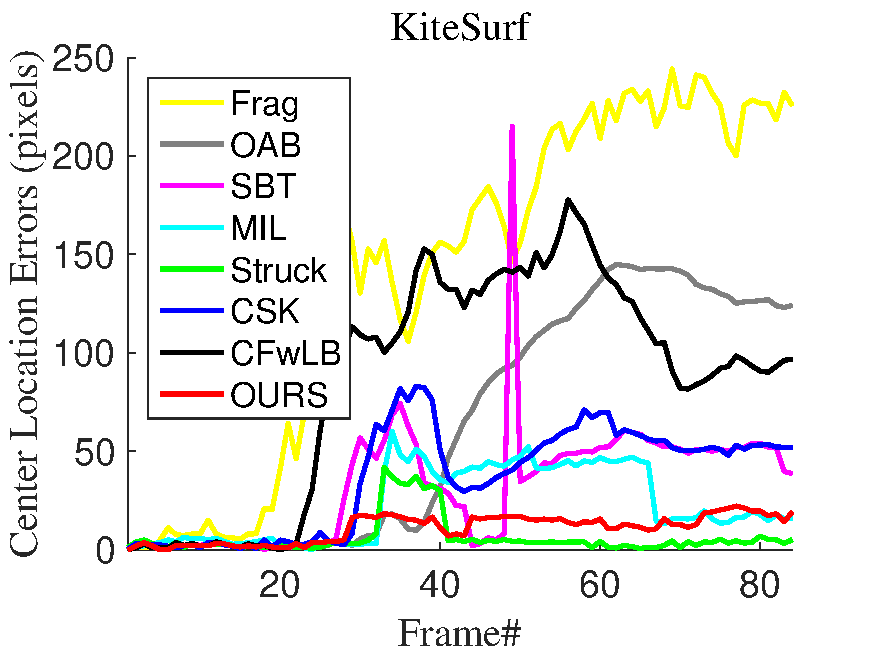
\includegraphics[width=0.3\linewidth]{CFwLB_KiteSurf_prcision.pdf}
\end{figure}
\end{frame}
\begin{frame}{中心位置误差对比}
\begin{figure}[htbp]
\centering
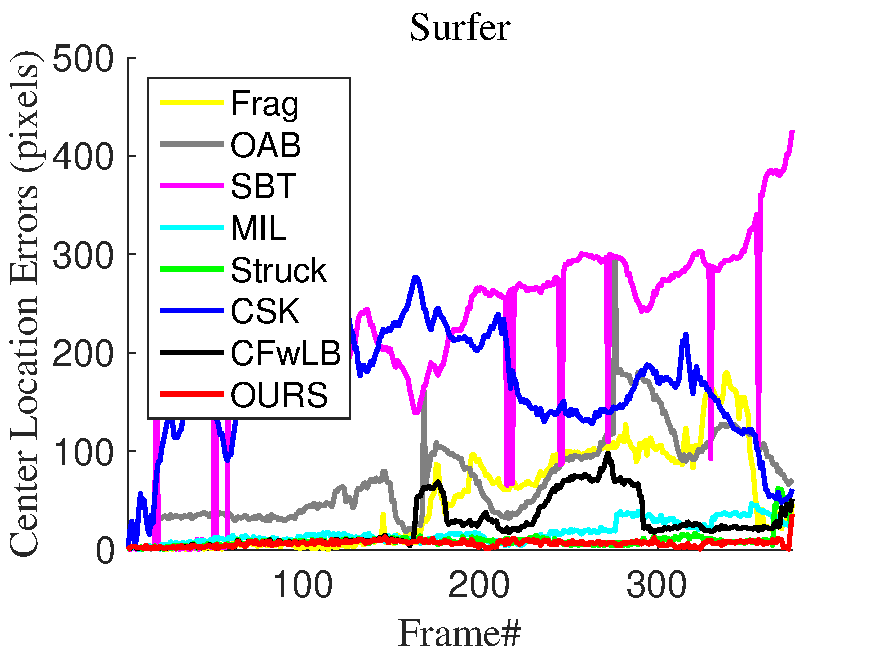
\includegraphics[width =0.3\linewidth]{CFwLB_Surfer_prcision.pdf}
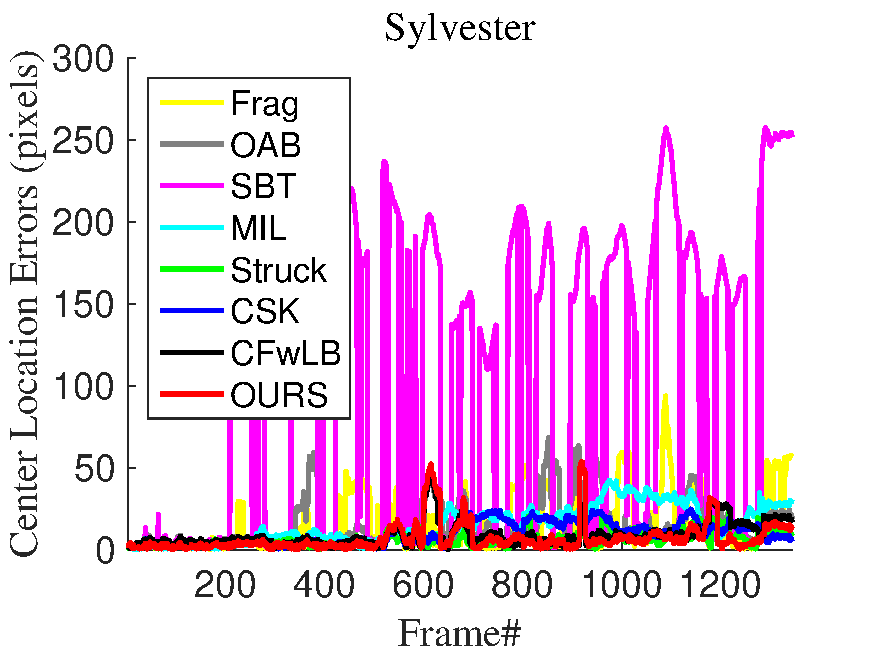
\includegraphics[width =0.3\linewidth]{CFwLB_Sylvester_prcision.pdf}
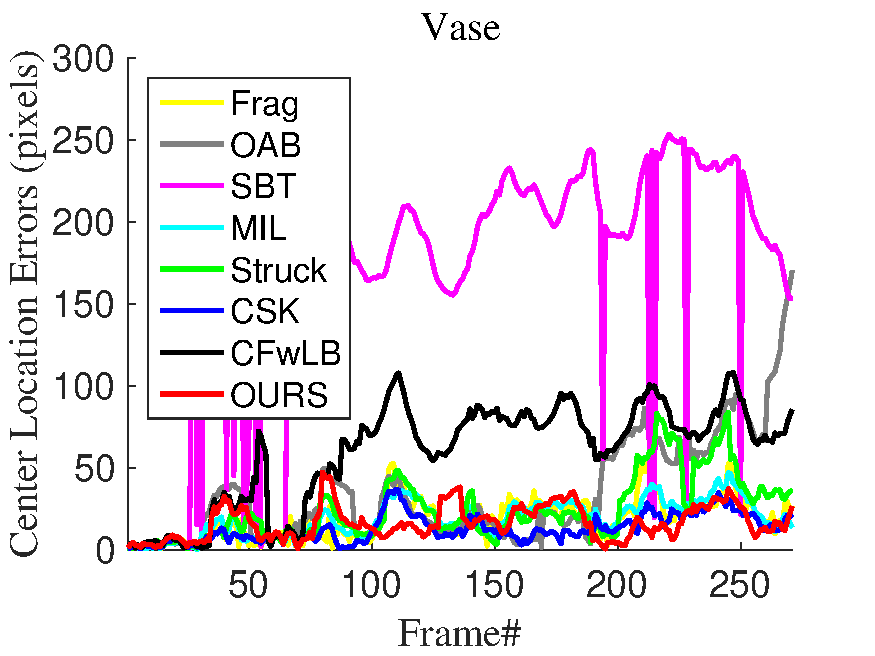
\includegraphics[width =0.3\linewidth]{CFwLB_Vase_prcision.pdf}
\end{figure}
\end{frame}

